\documentclass[11pt]{article}
\usepackage[margin=1in]{geometry}
\usepackage[T1]{fontenc}
\usepackage{lmodern}
\usepackage{amsmath,amssymb,amsthm}
\usepackage{booktabs}
\usepackage{graphicx}
\usepackage{xcolor}
\usepackage[numbers,sort&compress]{natbib}
\usepackage[colorlinks=true,linkcolor=blue!50!black,citecolor=blue!50!black,urlcolor=blue!50!black]{hyperref}

% generated by results/study2/make_paper_numbers.py: do not edit
\newcommand{\AblProfile}{smoke}
\newcommand{\BadRuns}{0}
\newcommand{\CalN}{200}
\newcommand{\CalTrials}{2000}
\newcommand{\DemoAcc}{7}
\newcommand{\DemoAnchor}{0.33}
\newcommand{\DemoBroken}{0}
\newcommand{\DemoChamp}{0.77}
\newcommand{\DemoCycles}{14}
\newcommand{\DemoFixed}{52}
\newcommand{\DemoGap}{0.43}
\newcommand{\DemoHeldA}{0.36}
\newcommand{\DemoHeldC}{0.36}
\newcommand{\DemoLedger}{verified}
\newcommand{\DemoRej}{5}
\newcommand{\DemoStep}{2}
\newcommand{\FASingle}{4.3}
\newcommand{\FATwo}{0.9}
\newcommand{\GainAOne}{+0.302}
\newcommand{\GainAThree}{+0.242}
\newcommand{\GainATwo}{-0.017}
\newcommand{\GainAZero}{+0.178}
\newcommand{\HFourMean}{0.000}
\newcommand{\HOneHi}{0.319}
\newcommand{\HOneHolm}{0.3047}
\newcommand{\HOneLo}{-0.076}
\newcommand{\HOneMean}{0.124}
\newcommand{\HOneP}{0.1523}
\newcommand{\HThreeHi}{0.066}
\newcommand{\HThreeHolm}{0.8438}
\newcommand{\HThreeLo}{-0.177}
\newcommand{\HThreeMean}{-0.064}
\newcommand{\HThreeP}{0.8438}
\newcommand{\HTwoHi}{0.272}
\newcommand{\HTwoHolm}{0.0117}
\newcommand{\HTwoLo}{0.120}
\newcommand{\HTwoMean}{0.195}
\newcommand{\HTwoP}{0.0039}
\newcommand{\HeldAOne}{+0.000}
\newcommand{\HeldAThree}{+0.000}
\newcommand{\HeldATwo}{+0.000}
\newcommand{\HeldAZero}{+0.000}
\newcommand{\HoneypotOK}{yes}
\newcommand{\KillFuzz}{211}
\newcommand{\KillMeta}{23}
\newcommand{\KillSmall}{203}
\newcommand{\MinP}{0.0039}
\newcommand{\MutAdj}{99.5}
\newcommand{\MutEquiv}{32}
\newcommand{\MutKilled}{215}
\newcommand{\MutN}{248}
\newcommand{\MutRate}{86.7}
\newcommand{\NCycles}{12}
\newcommand{\NSeeds}{8}
\newcommand{\OnlyFuzz}{12}
\newcommand{\OnlyMeta}{0}
\newcommand{\OnlySmall}{4}
\newcommand{\PowSingleOneZero}{100}
\newcommand{\PowSingleZeroEight}{95}
\newcommand{\PowSingleZeroFour}{52}
\newcommand{\PowSingleZeroSix}{80}
\newcommand{\PowSingleZeroTwo}{22}
\newcommand{\PowSingleZeroZero}{5}
\newcommand{\PowTwoOneZero}{99}
\newcommand{\PowTwoZeroEight}{94}
\newcommand{\PowTwoZeroFour}{40}
\newcommand{\PowTwoZeroSix}{75}
\newcommand{\PowTwoZeroTwo}{12}
\newcommand{\PowTwoZeroZero}{1}
\newcommand{\PreregHash}{b36d851de8d8}
\newcommand{\RefFalseFail}{0}
   % every number below that comes from an experiment is a macro generated from raw results

\newcommand{\repo}{\url{https://github.com/abdelkabirouadoukou/si-loop}}
\newtheorem{proposition}{Proposition}

\title{Guarded Recursive Self-Improvement:\\
Bounding Creeping Degradation and Reward Hacking in Autonomous Agent Loops}
\author{Abdelkabir Ouadoukou\thanks{Independent researcher. Contact: abdelkabir.ouadoukou@gmail.com.
This work was carried out with substantial AI assistance; see the disclosure at the end of the paper.}}
\date{November 2026 \\ \small Technical report (Study 2). Not peer reviewed.}

\begin{document}
\maketitle

\begin{abstract}
Agents that edit their own code can improve, but the usual loop (``propose a patch, keep it if a score goes up'') fails in
three ways: many individually harmless-looking patches add up to a regression (\emph{creeping degradation}), the
selection data is reused until the score no longer means anything (\emph{adaptive overfitting}), and the agent finds
ways to satisfy the checker instead of the task (\emph{reward hacking}). Study~1 added a second problem: a judge that is
too strict rejects almost everything. We treat self-improvement as a control problem and describe SI-Loop~v2, a kernel
that sits between a proposing agent and a sealed verifier. Its parts are: zero-trust git worktrees with a seven-layer patch
defence; a paired non-inferiority gate applied in two stages (a screen on batch~A with anytime-valid sequential stopping, then a
strict test on an independent batch~B) that removes the winner's curse; a frozen cycle-0 anchor with a finite \emph{margin budget}
that only proven gain can refill; a held-out problem family that selection never touches; a three-tier verifier with
honeypots and a measured mutation kill rate; a hash-chained ledger with circuit breakers; and pre-registered ablation arms
(A0 frozen improver, A1 full recursion, A2 random patches, A3 compute-matched best-of-N) to test whether recursion adds anything.
On a simulated null patch, the two-stage judge accepts \FATwo\% of patches at its default threshold, against \FASingle\% for a single stage, with a power loss that shrinks to about two points for a true gain of eight points. The verifier's tiers kill \MutRate\% of \MutN{} injected faults (\MutAdj\% after removing survivors that pass an extra-large fuzz run and are likely equivalent). In a pre-registered
pilot on a \emph{synthetic} world with \NSeeds{} seeds, we report the ablation results as they came out (Section~\ref{sec:abl}), including what the pilot cannot show. We also provide a
reference implementation with hidden pytest cases and an LLM meta-agent interface. We do \emph{not} claim recursive self-improvement of language models;
we claim a measurable, auditable harness in which such a claim could be tested.
\end{abstract}

\section{Introduction}

Systems that rewrite their own code are no longer hypothetical: the Darwin G\"odel Machine validates self-modifications
empirically \citep{zhang2025dgm}, hyperagents make the improvement procedure itself editable \citep{zhang2026hyperagents},
and the Huxley-G\"odel Machine argues that a parent should be judged by the productivity of its descendants, not its own score
\citep{wang2026hgm}; the classical formulation goes back to G\"odel machines \citep{schmidhuber2007godel}. Surveys cover the wider
landscape \citep{chen2026rsi}. These systems mostly rely on one signal (a benchmark score) and one rule (keep the patch if the score rises).
That is where the failures start.

\paragraph{Failure modes of the simple loop.}
\begin{itemize}\setlength\itemsep{0pt}
\item \textbf{Creeping degradation.} A gate that accepts any patch that is ``not significantly worse'' also accepts a patch that is
slightly worse. Each step passes; a hundred steps do not. Rewards for ``smaller'' or ``cheaper'' code make this path attractive.
\item \textbf{Adaptive overfitting.} Selecting among many patches on the same distribution inflates the measured gain
(winner's curse), and every reported number leaks information \citep{dwork2015holdout}.
\item \textbf{Reward hacking.} Proxy objectives are exploited when optimised hard \citep{gao2023scaling,coste2024ensembles}, and
self-play judges can be convinced \citep{zhou2026convincing}. For code agents this includes reading the tests, writing the result
file, or special-casing the checker.
\item \textbf{Over-conservative judging.} In Study~1 the guarded judge rejected about $73\%$ of rounds and the arm without a judge won.
Safety that blocks all progress is also a failure.
\item \textbf{Unmeasured recursion.} A rising curve does not show that improving the \emph{improver} helped. Without a frozen-improver
control, compute-matched sampling and random-patch baselines, ``recursive'' is a label.
\end{itemize}

\paragraph{Approach.} Prompting the agent to be careful is not a control. We instead put a kernel in front of the agent that the agent
cannot modify, make every acceptance a calibrated statistical decision on fresh data, bound the total slack the system may spend, keep one family of problems
completely out of the selection loop to measure generalisation, and measure the whole thing against pre-registered controls.

\paragraph{Contributions.}
(1) A two-stage, anytime-valid acceptance pipeline and its false-accept calibration (Sections~\ref{sec:gate}, \ref{sec:cal}).
(2) A margin budget and anchor audit that bound creeping degradation (Section~\ref{sec:budget}).
(3) A verifier design with three tiers, honeypots and a measured kill rate (Sections~\ref{sec:ver}, \ref{sec:mut}).
(4) A yield test for the improver, clade parent selection and an operator bandit (Section~\ref{sec:yield}).
(5) A tamper-evident ledger and circuit breakers for long runs (Section~\ref{sec:auto}).
(6) A pre-registered ablation runner and a reference implementation with an LLM interface (Sections~\ref{sec:ref}, \ref{sec:abl}).
Every component has prior art; our claim is the integration and the measurements, reported with their limits.

\section{Threat Model and Design Principles}
\label{sec:threat}

\paragraph{Adversary.} The meta-agent is untrusted: it may be buggy, over-optimising or actively trying to raise its score by illegitimate means.
It has read access to its own worktree and a token budget. It can submit one structured patch per cycle.
We do \emph{not} defend against an adversary with code execution outside the sandbox, with access to the verifier's secret, or against kernel bugs; local mode is not a security boundary.

\paragraph{Principles.}
(P1) \emph{Immutable kernel}: the code that judges is not in the code that is judged; a digest check aborts the run on any change.
(P2) \emph{Agents propose, the kernel disposes}: no direct writes; every change is a validated, atomic, reversible patch.
(P3) \emph{Fresh data for every decision}: problem ids are HMACs of a secret, per split and per cycle.
(P4) \emph{Coarse feedback}: the agent learns only accept / stepping\_stone / reject and a brief error type.
(P5) \emph{Bounded slack}: every non-proven accept spends from a finite budget; audits compare against a frozen reference.
(P6) \emph{Measure recursion against controls}, not against nothing.

\section{The SI-Loop v2 Architecture}
\label{sec:arch}

\begin{figure}[t]
\centering\small
\fbox{\parbox{0.92\linewidth}{\centering
\textbf{Immutable kernel} (digest-checked every cycle)\\
orchestrator $\to$ two-stage judge $\to$ gate $\to$ git promote / rollback;\\ ledger, circuit breakers, audits}}\\[2pt]
$\Big\downarrow$ \emph{proposal (strict JSON, AST scan, path policy)} \hspace{1.5em} $\Big\uparrow$ \emph{EvalResult only}\\[2pt]
\fbox{\parbox{0.44\linewidth}{\centering\textbf{Agent worktree}\\ \texttt{agent/**} is the only writable subtree; the meta-agent reads it and returns a proposal}}
\hspace{0.5em}
\fbox{\parbox{0.44\linewidth}{\centering\textbf{Sealed verifier}\\ secret, oracles, hidden tests, held-out family; candidate code runs in a separate sandbox process that gets inputs only}}
\caption{Trust boundaries. The agent never sees hidden tests, expected values, problem content, per-family numbers, counts, audit or held-out results.}
\label{fig:arch}
\end{figure}

\subsection{Zero-trust worktrees and the seven-layer patch defence}

Each cycle creates a git worktree from the chosen parent. The meta-agent returns a proposal; the kernel checks it through seven layers before
a single test runs (Table~\ref{tab:layers}). A proposal is a list of at most eight \emph{hunks}; each hunk is the unit of credit assignment.
The static scan is a first filter, not a security boundary: real isolation comes from the sandbox process (rlimits, scrubbed environment, no network, process-group kill; a container mode adds read-only root and \texttt{--network none}).

\begin{table}[t]
\centering\small
\caption{The seven layers applied to every patch.}
\label{tab:layers}
\begin{tabular}{cp{3.2cm}p{10.5cm}}\toprule
\# & Layer & What it rejects\\\midrule
1 & Strict parse & unknown keys, wrong types, more than 8 ops, oversize payloads, bad tags\\
2 & Path policy & anything outside \texttt{agent/}, traversal, dotfiles, \texttt{conftest.py}, other suffixes\\
3 & AST scan & forbidden imports (\texttt{socket}, \texttt{subprocess}, \texttt{ctypes}, \dots), \texttt{eval}/\texttt{exec}/\texttt{open}, dunder escapes, dangerous \texttt{os.*}\\
4 & Test ratchet & removed tests; \texttt{skip}, \texttt{xfail}, \texttt{importorskip}\\
5 & Atomic exact apply & ambiguous symbols; any failing op leaves the tree untouched\\
6 & Diff audit & committed files differing from the files named in the proposal\\
7 & Sandboxed self-tests & failing public tests, timeouts, memory blow-up\\\bottomrule
\end{tabular}
\end{table}

\subsection{The paired non-inferiority gate}
\label{sec:gate}

Parent and candidate run on the same fresh problems. Let $b$ be the number of problems the patch fixed, $c$ the number it broke, $n$ the number of problems, $\delta=(b-c)/n$,
$\mathrm{se}=\sqrt{b+c-(b-c)^2/n}\,/n$ and $\ell=\delta-z\,\mathrm{se}$ with $z=1.645$ (a normal approximation; the one-sided lower bound used for non-inferiority \citep{blackwelder1982}). With a flat prior on the fix probability among discordant pairs,
\[
p_{\mathrm{better}}=P\big(\mathrm{Bin}(b+c+1,\tfrac12)\le b\big).
\]
A patch is accepted if $\ell\ge-\varepsilon$, $\delta>0$ and $p_{\mathrm{better}}\ge p_{\min}$, or (utility path) if it is non-inferior and clearly smaller or cheaper.
A non-inferior, behaviourally novel patch becomes a \emph{stepping stone} (archived, not promoted); novelty can never rescue a regression.
The threshold $p_{\min}$ is chosen by A/A calibration for the batch size at hand (Section~\ref{sec:cal}).

\subsection{Two stages, sequential stopping and online FDR}
\label{sec:two}

\paragraph{Screen then confirm.} Batch~A (lenient, $p_{\mathrm{screen}}=0.80$) is evaluated in chunks. A candidate that passes is evaluated on an \emph{independent} batch~B, and the strict gate is applied to batch~B alone.
Because B was not used to select the candidate, the winner's curse does not apply to it; because both stages must pass, the false-accept probabilities multiply.

\paragraph{Anytime-valid early stopping.} After each chunk of A we update the discordant counts $(b,c)$. For harm we use the mixture e-value
\[
E_{\downarrow}=\frac{B(c+1,b+1)\sum_{k\le c}\binom{b+c+1}{k}}{1},\qquad \text{stop if } E_{\downarrow}\ge 1/\alpha_{\mathrm{harm}},
\]
the mirror of the improvement e-value $E_{\uparrow}=B(b+1,c+1)\sum_{k\le b}\binom{b+c+1}{k}$, which is a mixture over $q\sim U(\tfrac12,1)$ of the likelihood ratio $q^b(1-q)^c/(1/2)^{b+c}$ and hence an e-value under every null with fix probability $\le\tfrac12$.
By Ville's inequality \citep{ramdas2023gtsavi}, stopping at any data-dependent time keeps the error bound. For futility we use Wald's SPRT \citep{wald1945sprt} with alternative $p_1=\tfrac12+\theta$.
A stop only drops a candidate early; it cannot create an accept, because acceptance happens on B.

\paragraph{Online FDR.} Over thousands of cycles the number of accepts under the null grows. Confirmed accepts are optionally passed to e-LOND \citep{xu2024elond}, which controls the false discovery rate under arbitrary dependence; we run it in monitor mode (logged) or enforce mode (blocking).

\subsection{Anchor, margin budget and audits}
\label{sec:budget}

The champion at cycle~0 is frozen as the \emph{anchor}. Accepts that are not backed by a proven gain (the utility path) spend from a finite \emph{margin budget} $B_0$.
The charge of an accept with lower bound $\ell_i$ is $c_i=\max(\varepsilon_{\min},-\ell_i)$ (the amount of regression its bound could hide, with a floor). The budget is refilled only by a \emph{new high-water mark} of proven gain over the anchor, measured in audits on fresh batches.
Every $K$ cycles an audit compares the champion with the anchor and with its own historical peak and rolls back on regression.

\begin{proposition}[Budget bound]
Suppose utility-path accepts $i=1,\dots,k$ have true paired changes $\delta_i$ and lower bounds $\ell_i$ with $P(\delta_i\ge\ell_i)\ge1-\alpha$, and charges $c_i\ge\max(0,-\ell_i)$. On the event that all bounds hold (probability $\ge1-k\alpha$ by a union bound),
the total regression introduced by these accepts satisfies $\sum_i\max(0,-\delta_i)\le\sum_i c_i\le B_0+R$, where $R$ is the total refill, and $R$ is at most the proven gain over the anchor.
\end{proposition}
\begin{proof}[Sketch]
On the event, $-\delta_i\le-\ell_i\le c_i$ whenever $\delta_i<0$. Spending cannot exceed the balance, so $\sum c_i\le B_0+R$, and refills equal increments of a high-water mark of lower bounds on gain over the anchor. \qedhere
\end{proof}
The proposition is deliberately modest: it bounds the sum of step losses (not the net drift), assumes valid per-step bounds (ours are normal approximations), and ignores correlation between steps. The anchor audit is the backstop for exactly these gaps.

\subsection{Held-out family and noisy audits}

One problem family is drawn \emph{only} by the audit split. It is never used for selection, confirmation, credit, anchor or yield batches. The cross-family gap is
the selection gain minus the held-out gain of the champion against the anchor. Audit decisions that read reusable data are made through a Thresholdout-style noisy comparison \citep{dwork2015holdout}, and results are written to the ledger, never to the agent.
A large gap pauses the run.

\subsection{Sealed verifier: three tiers, honeypots, mutation testing}
\label{sec:ver}

Every problem is checked by three tiers: small-scope exhaustive inputs, random large-scope fuzzing, and metamorphic invariance relations (for example, adding spaces around operators must not change an arithmetic result).
The oracle and the comparison run in the judge; candidate code runs in a sandbox worker. Honeypots are impossible problems with junk expectations that exist only in decoy files; passing one, opening a decoy path, or emitting a canary sets a security flag and an automatic reject, and the commit is quarantined.
To measure the verifier itself we apply AST mutations (comparison swaps, operator swaps, constant changes, deleted statements, \texttt{return None}) to known-correct reference solutions and count how many mutants the tiers reject \citep{demillo1978mutation,jia2011mutation}. Survivors that also survive an extra-large fuzz run are counted as likely equivalent mutants.

\subsection{Yield testing, clades and the operator bandit}
\label{sec:yield}

A patch that edits the improver (\texttt{agent/meta/**}) changes how future patches are made, so a solver score cannot judge it. We evaluate its \emph{yield}: the gain in pass rate after $K$ inner cycles on a fresh batch,
from identical start states and seeds, for the candidate improver, its parent, and the frozen reference improver M0. It is accepted iff the bootstrap lower bound of the paired yield difference to the parent is positive and the yield is not worse than M0 by more than a tolerance.
Mixed-scope patches are rejected. Parents are chosen by Thompson sampling on discounted descendant successes (clade productivity, after \citealp{wang2026hgm}), not by their own score. An operator bandit tracks an exponential moving average of reward per hunk tag.

\subsection{Long-run autonomy}
\label{sec:auto}

The ledger is append-only and hash-chained: $h_t=\mathrm{SHA256}(h_{t-1}\Vert\mathrm{canon}(r_t))$, so any edit of history is detected on verification. Circuit breakers trip on: accept-rate anomalies (binomial tail against a pre-registered rate), LOC explosions, cost spikes, repeated sandbox-escape attempts, security flags and repeated audit regressions;
a trip pauses or latches a HALT file. A heartbeat and an external watchdog cover a silent crash; a model and kernel fingerprint is logged and a change halts the run because it invalidates calibration. Orphan worktrees and stale branches are garbage-collected.

\section{Reference Implementation}
\label{sec:ref}

Two reviewer concerns about earlier drafts were that the verifier and the meta-agent were only interfaces. The repository now contains a complete reference pair.

\paragraph{Task suite and hidden pytest.} \texttt{study2/} defines 15 tasks in three families: string (6), algorithmic (6) and a held-out parsing family (3). Each has a public specification (a docstring), a judge-side oracle and a case generator that mixes ordinary and edge-case inputs. The seed agent has about half of the functions buggy or missing.
For each evaluation the judge derives the tasks from HMAC-based ids, copies the candidate's \texttt{agent/} into a sandbox process that receives \emph{inputs only}, collects the outputs, writes a hidden pytest file with expected and actual values, and runs pytest in its own process. A problem passes iff its pytest test passes on all six cases.
Because candidate code never shares a process with pytest or an oracle, it cannot patch the test runner or read an expected value; a forged result without the per-run nonce is ignored, and a decoy file tripwire flags attempts to read ``hidden'' paths. A separate self-check confirms that a library of oracle solutions passes $100\%$ (no false rejects).

\paragraph{LLM meta-agent.} \texttt{LLMMetaAgent} builds a prompt from the agent's own source and untrusted lessons, asks for a JSON proposal, parses it with the kernel's strict \texttt{parse\_proposal}, and retries malformed replies with the error text; all calls are charged to the cycle's token budget.
Clients exist for any OpenAI-compatible endpoint (a local Ollama, vLLM, llama.cpp or LM Studio server, or OpenAI) and for the Anthropic API, plus a scripted offline client used for tests and demos. \texttt{run\_study2.py} wires everything together (\texttt{check}, \texttt{demo}, \texttt{run}, \texttt{report}).

\section{Evaluation}
\label{sec:eval}

We separate what is measured from what is only demonstrated. Sections~\ref{sec:cal} and \ref{sec:mut} are measurements of components. Section~\ref{sec:demo} demonstrates the pipeline with a scripted proposer. Section~\ref{sec:abl} is a pre-registered pilot on a synthetic world.

\subsection{False-accept calibration and power}
\label{sec:cal}

We simulate A/A tests: both versions have the same true pass rate $p=0.5$, with independent run-to-run noise ($\sigma=0.1$ on the latent scale), $n=\CalN$ problems per batch and \CalTrials{} trials per setting (power uses $1000$).
At $p_{\min}=0.95$ the single-stage gate accepts \FASingle\% of null patches and the two-stage judge \FATwo\%. Figure~\ref{fig:cal} and Table~\ref{tab:cal} show the full curves.
The price is power: for a patch that truly adds $2$, $4$, $6$, $8$ points of pass rate, the single stage accepts \PowSingleZeroTwo\%, \PowSingleZeroFour\%, \PowSingleZeroSix\%, \PowSingleZeroEight\% and the two-stage judge \PowTwoZeroTwo\%, \PowTwoZeroFour\%, \PowTwoZeroSix\%, \PowTwoZeroEight\%.
Small true gains are therefore the ones that are lost, which is the intended trade: they are also the ones most easily produced by noise.
The noise model is an assumption; estimate the real run-to-run noise from repeated evaluations of an unchanged agent before trusting these numbers.

\begin{figure}[t]
\centering
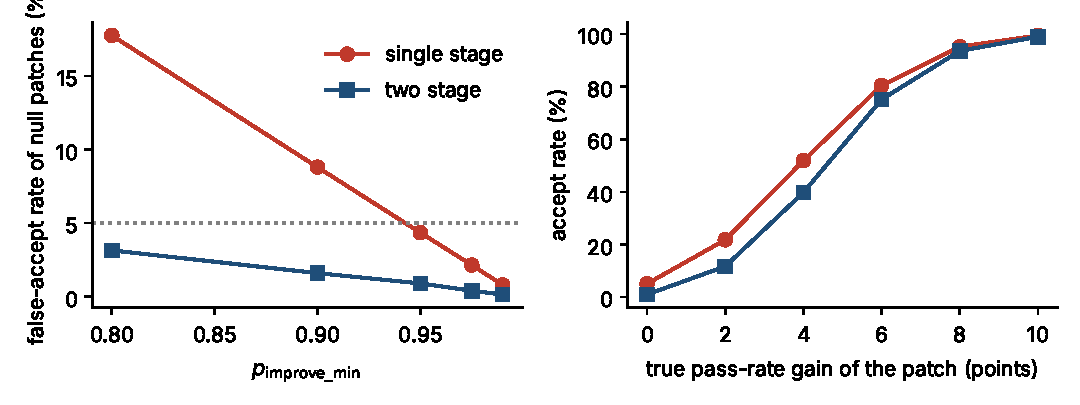
\includegraphics[width=0.95\linewidth]{results/study2/fig_calibration.pdf}
\caption{Left: false-accept rate of null patches against $p_{\mathrm{improve\_min}}$. Right: accept rate against the true gain (at $p_{\mathrm{improve\_min}}=0.95$).}
\label{fig:cal}
\end{figure}

\begin{table}[t]
\centering\small
\caption{A/A false-accept rate ($n=\CalN$, $p=0.5$, $\sigma=0.1$).}
\label{tab:cal}
\begin{tabular}{lcc}\toprule
$p_{\mathrm{improve\_min}}$ & single stage & two stage \\\midrule
0.800 & 17.8\% & 3.1\% \\
0.900 & 8.8\% & 1.6\% \\
0.950 & 4.3\% & 0.9\% \\
0.975 & 2.1\% & 0.4\% \\
0.990 & 0.8\% & 0.1\% \\
\bottomrule\end{tabular}
\end{table}

\subsection{Verifier quality}
\label{sec:mut}

On the synthetic world's nine sealed task kinds we generated \MutN{} mutants of the reference solutions; the three tiers killed \MutKilled{}: a raw kill rate of \MutRate\%. Of the survivors, \MutEquiv{} also passed an extra-large fuzz run and are treated as likely equivalent mutants (for example, edits to code paths that the sampled parameters never reach), giving \MutAdj\%. The ``equivalent'' label is a heuristic, not a proof, so the raw rate is the conservative figure.
Kills by tier were small-scope \KillSmall, fuzz \KillFuzz, metamorphic \KillMeta; mutants killed \emph{only} by one tier were \OnlySmall, \OnlyFuzz{} and \OnlyMeta{} respectively, which is each tier's marginal value. In this suite the metamorphic tier killed no mutant that the other tiers missed; its value here is limited to the arithmetic kinds, where it targets tokenisation-style bugs that small-scope tests can miss. We keep it because a kill rate on injected faults does not measure the faults we did not inject.
The correct reference solutions failed $\RefFalseFail$ times (they must never fail), and the planted snooping solver was detected: \HoneypotOK.
The adjusted rate is evidence about the injected-fault class only; it does not bound the probability of a verifier gap an LLM would find.

\subsection{End-to-end pipeline run (scripted proposer)}
\label{sec:demo}

\texttt{run\_study2.py demo} runs \DemoCycles{} cycles of the reference implementation with a \emph{scripted} proposer (a list of fixes, one deliberate regression, one deliberately malformed reply); it is not a language model and demonstrates the machinery only.
Of the \DemoCycles{} cycles, \DemoAcc{} were accepted, \DemoStep{} were stepping stones and \DemoRej{} were rejected; the hash chain of the ledger was \DemoLedger. On fresh batches the champion's pass rate on the selection families rose from \DemoAnchor{} (anchor) to \DemoChamp{}
(\DemoFixed{} problems fixed, \DemoBroken{} broken out of $120$), while the held-out family stayed at \DemoHeldA{} $\to$ \DemoHeldC{}. The cross-family gap of \DemoGap{} raised the generalisation alarm, as it should: the scripted proposer fixes only functions in the selection families.
The deliberate regression (a function returning $0$) was stopped by the sandboxed self-tests, and the malformed reply was retried.

\subsection{Pre-registered ablation pilot}
\label{sec:abl}

\paragraph{Design.} The unit of analysis is the run (seed). Arms: A0 frozen improver (solver patches only), A1 full recursion (solver and improver, improver judged by yield tests), A2 random-patch control, A3 compute-matched best-of-N
(every proposal is made from the anchor and the champion is the best single patch). Each arm runs \NCycles{} cycles on \NSeeds{} seeds in the \AblProfile{} profile; final evaluation uses fresh batches shared by every arm and seed.
Hypotheses are fixed before the runs: H1 A1$>$A0 on final selection gain; H2 A0$>$A2; H3 A0$>$A3 (one-sided paired sign-flip tests, Holm-corrected over H1--H3); H4 A1$-$A0 on held-out gain $\ge-0.02$.
The pre-registration (hash \PreregHash\dots) is locked to the kernel digest; the runner refuses to start if either changes. With \NSeeds{} seeds the smallest attainable one-sided p-value is \MinP.
The world is synthetic: the ``meta-agent'' is a seeded mutation engine, so A1 tests whether tuning the \emph{policy} of such an engine helps. It tests the harness, not an LLM.

% ABLATION-PROSE-START
\paragraph{Results.} Table~\ref{tab:abl} and Table~\ref{tab:tests} are generated from the raw per-run files. No run halted, tripped a security flag or broke the ledger (\BadRuns{} such runs). The mean final gain on the selection families over the frozen cycle-0 anchor was \GainAZero{} (A0), \GainAOne{} (A1), \GainATwo{} (A2) and \GainAThree{} (A3).

\begin{table}[t]
\centering\small
\caption{Arms, mean $\pm$ SD over seeds. Gain is the final pass rate minus the anchor's, on fresh batches shared by all arms. Tokens include yield tests.}
\label{tab:abl}
\begin{tabular}{lcccrr}\toprule
Arm & seeds & gain, selection families & gain, held-out & accepts & tokens \\\midrule
A0 & 8 & $+0.178\pm0.129$ & $+0.000$ & 1.5 & 12,534 \\
A1 & 8 & $+0.302\pm0.220$ & $+0.000$ & 1.8 & 29,098 \\
A2 & 8 & $-0.017\pm0.018$ & $+0.000$ & 2.6 & 11,776 \\
A3 & 8 & $+0.242\pm0.122$ & $+0.000$ & 1.0 & 12,429 \\
\bottomrule\end{tabular}
\end{table}

\begin{table}[t]
\centering\small
\caption{Pre-registered contrasts (paired by seed; one-sided sign-flip p; Holm over H1--H3).}
\label{tab:tests}
\begin{tabular}{llcccrr}\toprule
Hyp. & contrast & pairs & mean diff. & 95\% bootstrap CI & p (one-sided) & Holm p \\\midrule
H1 & A1$-$A0 & 8 & $+0.124$ & $[-0.076,+0.319]$ & 0.1523 & 0.3047 \\
H2 & A0$-$A2 & 8 & $+0.195$ & $[+0.120,+0.272]$ & 0.0039 & 0.0117 \\
H3 & A0$-$A3 & 8 & $-0.064$ & $[-0.177,+0.066]$ & 0.8438 & 0.8438 \\
\bottomrule\end{tabular}
\end{table}

\begin{itemize}\setlength\itemsep{2pt}
\item \textbf{H2 supported} (A0$-$A2 $=$ \HTwoMean{}, Holm $p=$ \HTwoHolm). Random patches behind the same gate did not improve the agent (\GainATwo{}), while informed proposals behind the same gate did. The gain is therefore not an artefact of the gate or of the evaluation. The gate also kept the random arm from degrading: its mean loss was small, but not zero (below).
\item \textbf{H1 not supported} (A1$-$A0 $=$ \HOneMean{}, 95\% CI $[$\HOneLo{}, \HOneHi{}$]$, Holm $p=$ \HOneHolm). The point estimate favours A1, but the interval includes zero. More importantly, \emph{no improver patch was accepted in any A1 run}: 13 improver patches were proposed across the eight runs and none was accepted. A1 and A0 therefore ran the same improver policy except that A1 spent about $15\%$ of its proposals on (rejected) policy edits. The positive difference reflects run-to-run variation of the proposal stream (A1's per-seed gains are bimodal), not recursion. This pilot cannot say anything about whether improving the improver helps.
\item \textbf{H3 not supported} (A0$-$A3 $=$ \HThreeMean{}, Holm $p=$ \HThreeHolm). Compute-matched best-of-N from the anchor (\GainAThree{}) was at least as good as iterating and accumulating (\GainAZero{}). In this small world each useful fix is independent, so iteration adds nothing over sampling. A1 used about $2.3\times$ the tokens of the other arms because of yield tests (Table~\ref{tab:abl}); A1 vs.\ A3 was not pre-registered and is not tested.
\item \textbf{H4 is uninformative.} The held-out gain was \HeldAZero{} in every arm because the toy improver never edits the interpreter family; the non-inferiority margin held trivially. The held-out audit machinery is exercised in the end-to-end run (Section~\ref{sec:demo}), but this ablation provides no evidence about cross-family overfitting.
\end{itemize}

\paragraph{The random arm and the margin budget.} A2 accepted $2.6$ patches per run on average. Its final gain ranged from $-0.052$ to $0.000$ (mean \GainATwo{}); the margin spent per run ranged from $0.005$ to $0.020$ against a budget of $0.03$. The worst run lost $0.052$ on the final batch while having spent only $0.005$.
That is a counter-example to reading the budget as a hard bound on true loss: the charge is a lower-bound-based estimate, the final batch ($96$ problems) is itself noisy (standard error roughly $0.02$), and the proposition holds only when the per-step bounds hold. What the data do support is narrower: with the budget and floor in place, a policy that proposes random edits lost about two points on average and no more than five in the worst of eight runs, and never gained.

\paragraph{What this pilot does and does not show.} It shows that the harness runs end to end under pre-registration, that the gate separates informed from random search (H2), and that the controls (A2, A3) are needed: without A3, the gain of A0 or A1 would have been read as evidence for iteration. It does not show recursive self-improvement; the one test of it (H1) is empty because the improver never changed. With \NSeeds{} seeds the smallest attainable one-sided p-value is \MinP{}, so only large, consistent effects could be detected. A real study needs more seeds, a world in which improver edits can matter, and an LLM meta-agent.

% ABLATION-PROSE-END

\section{Discussion and Limitations}

\paragraph{Adaptive overfitting.} The two-stage design removes the winner's curse for each decision, and fresh HMAC batches prevent reuse, but over many cycles the agent can still adapt to the \emph{distribution} (families, edge-case style) through accepted code.
Coarse feedback limits leakage rather than eliminating it; the held-out family is the detector, and it only detects generalisation failure across families we thought of. The scripted run shows the alarm firing; whether an LLM would overfit is an open empirical question.

\paragraph{Verifier quality.} Mutation kill rate measures sensitivity to simple injected faults. It says little about semantic loopholes (an under-specified oracle, a missing edge-case family). Honeypots catch curiosity, not stealth.
Every verifier needs red-teaming by an adversarial model before a claim of ``no reward hacking'' is made.

\paragraph{Margin budget.} The proposition is conditional and bounds a sum, not drift; underestimated charges are possible. The budget makes creep expensive and visible, and the audit makes it reversible, but neither makes it impossible.

\paragraph{Synthetic mutation engine versus real LLM meta-agents.} Our ablation uses a simulated improver because it is deterministic, free and fast; its dynamics (a handful of operators, a library of fixes) are far from an LLM's. The step from simulation to a model is where most of the uncertainty lies: proposals become much more varied, token costs matter, failure modes include prompt injection through source comments,
and run-to-run noise rises, so batch sizes and $p_{\min}$ must be recalibrated. The kernel does not change; the calibration, the budgets, the number of seeds and the cost of yield tests do. We provide the interface (\texttt{LLMMetaAgent}) and a local-model path, but report no LLM results here.

\paragraph{Other limits.} Container mode is untested; the local sandbox is not a security boundary. Cost is counted in LOC and tokens, not deterministic instructions. The pilot has few seeds and a small world. The judge's normal-approximation lower bound is not exact for small discordant counts.
Several references in \texttt{references.bib} are marked FROM-KNOWLEDGE and must be checked before submission.

\section{Conclusion and Reproducibility}

Guarding self-improvement is mostly bookkeeping: who may write, which data decides, how much slack remains, what was measured against which control. SI-Loop~v2 puts that bookkeeping in an immutable kernel, calibrates its acceptance rule, and ships a pre-registered harness for asking whether recursion helps. The next step is the one this paper does not take: running it with a real LLM meta-agent, with the calibration and seeds this setting requires.

\paragraph{Reproducibility.} Code and data: \repo. Tests: \texttt{python -m pytest -q tests}. Verifier self-check: \texttt{python run\_study2.py check}. Demo: \texttt{python run\_study2.py demo}. Calibration: \texttt{python results/study2/make\_calibration.py}.
Verifier quality: \texttt{python -m kernel.mutation}. Ablations: \texttt{python run\_ablations.py prereg|run|analyze}. All numbers and tables in Section~\ref{sec:eval} are generated by \texttt{results/study2/make\_paper\_numbers.py} from the raw result files in \texttt{results/study2/}.
Study~1 is frozen and unchanged; \texttt{si\_loop\_toy.py} is pinned by hash in \texttt{results/config\_hashes.txt}.

\paragraph{AI assistance disclosure.} The code, the experiments' scripts and the drafting of this report were produced with substantial assistance from an AI system (Anthropic's Claude), under the author's direction.
The author decided the study design and is responsible for the content. Numerical values come from generated files; references marked FROM-KNOWLEDGE in the bibliography were not re-fetched.

\bibliographystyle{plainnat}
\bibliography{references}

\end{document}
